\documentclass{beamer}
\usetheme{Madrid}
%\setbeamertemplate{page number in head/foot}{}
\usepackage{dirtytalk}
\usepackage{listings}
\usepackage{graphicx}
\usepackage{caption}
\usepackage{stmaryrd}
\usepackage{color}
\definecolor{lightgray}{rgb}{.9,.9,.9}
\definecolor{darkgray}{rgb}{.4,.4,.4}
\definecolor{purple}{rgb}{0.65, 0.12, 0.82}
\lstdefinelanguage{Solidity}{
  keywords={break, case, catch, continue, debugger, default, delete, do, else, false, finally, for, function, if, in, instanceof, new, null, return, switch, this, throw, true, try, typeof, var, void, while, with},
  morecomment=[l]{//},
  morecomment=[s]{/*}{*/},
  morestring=[b]',
  morestring=[b]",
  ndkeywords={contract, export, boolean, throw, implements, import, this},
  keywordstyle=\color{blue}\bfseries,
  ndkeywordstyle=\color{darkgray}\bfseries,
  identifierstyle=\color{black},
  commentstyle=\color{darkgray}\ttfamily,
  stringstyle=\color{red}\ttfamily,
  sensitive=true,
}

\lstdefinestyle{transitions}{
    language={Solidity},
    moredelim=**[is][\only<2->{\color{red}}]{@}{@},
}

\lstdefinelanguage{Solar}{
  keywords={uses,matches,interefere,where},
  ndkeywords={Transfer,Argument,Store},
  keywordstyle=\color{blue}\bfseries,
  ndkeywordstyle=\color{darkgray}\bfseries,
  identifierstyle=\color{black},
  commentstyle=\color{darkgray}\ttfamily,
  stringstyle=\color{red}\ttfamily,
  sensitive=true,
  mathescape=true
}


\lstdefinelanguage{Racket}{
  keywords={define,when,match},
  ndkeywords={where},
  keywordstyle=\color{blue}\bfseries,
  ndkeywordstyle=\color{darkgray}\bfseries,
  identifierstyle=\color{black},
  commentstyle=\color{darkgray}\ttfamily,
  stringstyle=\color{red}\ttfamily,
  sensitive=true,
  mathescape=true
}

\lstset{
   language=Solidity,
   extendedchars=true,
   basicstyle=\tiny\ttfamily,
   showstringspaces=false,
   showspaces=false,
   numbers=left,
   numberstyle=\footnotesize,
   numbersep=9pt,
   tabsize=2,
   breaklines=true,
   showtabs=false,
   captionpos=b
}
\lstdefinelanguage{account}{
  keywords={balance, storage, code},
  morecomment=[l]{//},
  morecomment=[s]{/*}{*/},
  basicstyle=\tiny\ttfamily,
  morestring=[b]',
  morestring=[b]",
  ndkeywords={done},
  keywordstyle=\color{blue}\bfseries,
  ndkeywordstyle=\color{darkgray}\bfseries,
  identifierstyle=\color{black},
  commentstyle=\color{darkgray}\ttfamily,
  stringstyle=\color{red}\ttfamily,
  sensitive=true,
  framexleftmargin=0mm,
  frame=shadowbox,
  showstringspaces=false,
  numbers=none,
  xleftmargin=0cm,
  mathescape=true,
  framesep=0pt
}

\captionsetup[figure]{labelformat=empty}
\newcommand{\hole}{\textit{choose}}
\newcommand{\boldIt}[1]{\textbf{\textit{#1}}}
\newcommand{\vect}[1]{\overrightarrow{#1}}
\newcommand{\transfer}{\overline{\textit{transfer}}}
\newcommand{\sstore}{\overline{\textit{sstore}}}
\usefonttheme[onlymath]{serif}
\graphicspath{{./images/}}

%Information to be included in the title page:
\title[]{Summary-Based Symbolic Execution for Smart Contracts (ASE'20)}
\subtitle{Yu Feng, Emina Torlak \& Ratislav Bodik}
\author{Manasvi Saxena}

\setbeamerfont{caption}{size=\scriptsize}
\date{}
\begin{document}

\frame{\titlepage}

\section{Introduction}

\begin{frame}
  \frametitle{Motivation}
  \begin{itemize}
    \item \textit{Smart Contracts} find increasing adoption.
      Ethereum has ~45M contracts in
      \textit{finance}, \textit{gaming}, \textit{e-commerce}.
    \item Code on the blockchain \textit{immutable}. Critical
      issues cannot be \textit{patched} after deployment.
    \item Successful attacks have serious consequences:
      \begin{itemize}
        \item In 2016 \textit{Reentrace} bug lead to loss of ~\$150M and a hard
          fork.
        \item In 2017, \textit{Incorrect Permissions} lead to a loss of ~\$30M
        \item In 2018, \textit{Overflow} errors caused multiple tokens to shutdown
      \end{itemize}
  \end{itemize}
\end{frame}

\begin{frame}
  \frametitle{Challenges}
  \begin{itemize}
    \item Vulnerabilities may be \textit{intra}-contract or
      \textit{inter}-contract.
      \begin{itemize}
        \item Need to analyze both contract and
          interations with external accounts.
      \end{itemize}
    \item Multiple High Level Languages (Solidity, Vyper) compile to a
      stack based instruction set (EVM)
      \begin{itemize}
        \item Rapidly evolving ecosytem makes \textit{platform indepenence}
          important.
      \end{itemize}
    \item Widespread adoption requires a balance of
      \textit{strong guarantees}, \textit{ease of use} and \textit{automation}
      \begin{itemize}
        \item Verification may not be feasible due to lack of expertise
      \end{itemize}
    \item \textit{Configurable} and \textit{scalable} to detect multiple kinds of bugs
      in non-trivial contracts
      \begin{itemize}
        \item Checking for common anti-patterns alongside
          tests increase confidence in correctness
        \item Performance should not act as a bottleneck
          in development cycle.
      \end{itemize}
  \end{itemize}
\end{frame}


\begin{frame}
  \frametitle{Contributions}
  \textit{SOLAR} Synthesis tool for adversarial contracts
  to expose vulnerabilities
  \begin{itemize}
    \item Uses \say{Summary-Based Symbolic Execution} for \textit{Scalablity}
    \begin{itemize}
      \item Summaries drastically cuts execution instructions
    \end{itemize}
    \item Handles \textit{inter-contract} interactions
    \item Mostly \textit{automated}, though may require intervention
      in some cases
    \item Can be configured to detect different classes of vulnerabilities.
   \item \textit{Platform Independent} as it works over the bytecode
      instead of HLL like \textit{Solidity}, \textit{Serpent}
  \end{itemize}
\end{frame}

\section{Background}
\subsection{Smart Contracts and EVM}
\begin{frame}
  \frametitle{Background}
  \begin{block}{Smart Contracts}
    \begin{itemize}
      \item Program on second generation blockchains that are executed
        during transactions.
      \item Accounts have \textit{persistent storage} and hold \textit{coins}.
    \end{itemize}
  \end{block}
  \pause
  \begin{block}{Ethereum}
    \begin{itemize}
      \item \textit{Ethereum Virtual Machine} Network nodes
        understand a low level stack based language called \textit{EVM}
      \item Contracts written in High Level Languages (HLL) and compiled to EVM.
      \item The \textit{ABI} specifies convention for calling a contract
    \end{itemize}
  \end{block}
\end{frame}

\subsection{Examples}
\begin{frame}[fragile]
  \frametitle{Reentrace Vulnerability}
  \begin{columns}
    \begin{column}{0.5\textwidth}
      \begin{lstlisting}[numbers = none, language=Solidity, style=transitions]
      contract Victim {
        // ...
        function withdraw(unit a) {
          if(balances[msg.sender] >= a) {
            @msg.sender.call.value(a);@
            balances[msg.sender] -= a;
          }
        }
      }
      \end{lstlisting}
    \end{column}

    \begin{column}{0.5\textwidth}
      \begin{lstlisting}[language=Solidity, style=transitions, numbers=none]
      contract Attacker {
        Victim v;

        function exploit() {
          v = Victim(0x123);
          v.withdraw();
        }

        function payable() {
          @v.withdraw(10);@
        }
      }
      \end{lstlisting}
    \end{column}
  \end{columns}
  \begin{itemize}
    \item<2-> Within \textit{payable}, attacker calls \textit{withdraw}
      before victim updates persistent storage
    \item<2-> Trace \textit{transfer,transfer, ..., sstore} observed
  \end{itemize}

\end{frame}

\begin{frame}[fragile]
  \frametitle{Detection with SOLAR}
  Inputs to SOLAR - \textit{Attack template} and a \textit{Query}

  \begin{columns}[T]
    \begin{column}{0.4\textwidth}
      \center{\scriptsize{\textbf{Attack Template}}}
      \begin{lstlisting}[language=Solidity, style=transitions, numbers=none]
      contract Attacker {
        Victim v;

        function exploit() {
          v = Victim(0x123);
          ?? // Hole
        }

        function payable() {
          ?? // Hole
        }
      }
      \end{lstlisting}
    \end{column}
      \pause
    \begin{column}{0.6\textwidth}
      \center{\scriptsize{\textbf{Query}}}
      \begin{lstlisting}[language=Solar, numbers=none]
        uses Transfer $t_1$, $t_2$; Store s; Argument a;
        matches {$t_1$; ~s; $t_2$}
          where ($t_1$.loc == $t_2$.loc)
            $\wedge$ ($t_2$.gas > 2300)
            $\wedge$ (interfere? a $t_2$.reciepient)
      \end{lstlisting}
    \end{column}
  \end{columns}
  \pause
  \begin{itemize}
    \item \scriptsize{SOLAR Synthesizes a \textit{Concrete Attack Program} that
      satisfies \textit{Query}}.
    \item \scriptsize{\textit{Holes} in the \textit{Template} replaced with
      \textit{ABI calls} that satisfy \textit{Query}.}
\end{itemize}
\end{frame}
\subsection{SOLAR Overview}
\begin{frame}
  \frametitle{SOLAR Overview}
  SOLAR's synthesis works as following:
  \begin{itemize}
    \item Encode holes as \textit{choose statements} $\hole(\tau_1, \tau_2, \dots, \tau_n)$
      where $\tau_i$ is a tuple of the name and argument types
      of a method in the victim.
    \item The attack program is a sequence of $k$ statements.
      For $n$ public victim methods, SOLAR considers $n^k$
      programs.
    \item Symbolically executes the attack program on a state
      where victim identifier are bound to \textit{fresh variables}.
    \item Attempts to find a concrete call statements that satisfy \textit{Query}

  \end{itemize}
\end{frame}
\begin{frame}
  \frametitle{SOLAR Optimizations}
  SOLAR uses two optimizations:
      \begin{itemize}
        \item \textbf{Hoisting}
        \begin{itemize}
          \item $\hole(\tau_1, \tau_2)$ is sugar for
            $\text{if}(b_i) \tau_1 \text{else} \tau_2$,
            where $b_i$ is bound to a fresh variable.
          \item SOLAR \textit{hoists} over \textit{choose statements} by
            enumerating all possible attack programs.
          \item \textit{Hoisted} programs can be executed concurrently
      \end{itemize}
    \item \textbf{Summary Based Execution}
      \begin{itemize}
        \item SOLAR calculates \textit{summaries} for victim's
          methods for symbolic execution
      \end{itemize}
  \end{itemize}
\end{frame}


\section{Problem Formalization}
\subsection{SOLAR Language}
\begin{frame}
  \frametitle{SOLAR Intermediate Representation}
  \begin{columns}[T]
    \begin{column}{0.5\textwidth}
      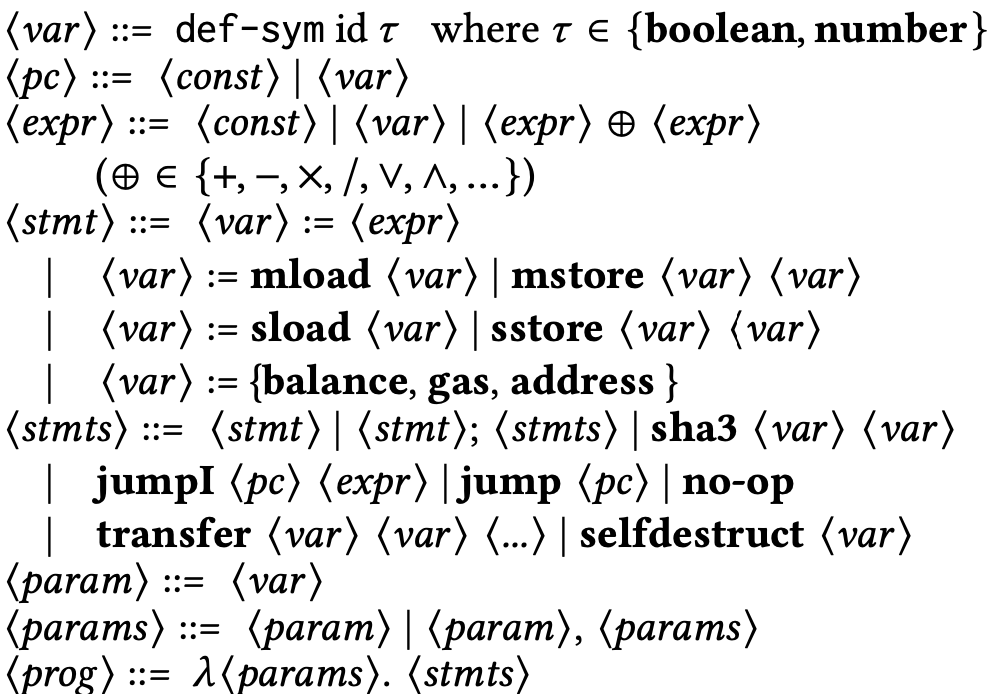
\includegraphics[scale=0.35]{IRGrammar}
    \end{column}
    \pause
    \begin{column}{0.5\textwidth}
      \begin{itemize}
      \item SOLAR IR is a superset of EVM
      \item Adds assignments, functions and symbolic
        variables
      \end{itemize}
    \end{column}
  \end{columns}
\end{frame}

\begin{frame}[fragile]
  \frametitle{SOLAR Query Language}
  \begin{columns}[T]
    \begin{column}{0.5\textwidth}
      \begin{lstlisting}[language=Solar, numbers=none]
        uses Transfer $t_1$, $t_2$; Store s; Argument a;
        matches {$t_1$; ~s; $t_2$}
          where ($t_1$.loc == $t_2$.loc)
            $\wedge$ ($t_2$.gas > 2300)
            $\wedge$ (interfere? a $t_2$.reciepient)
      \end{lstlisting}
    \end{column}
    \begin{column}{0.5\textwidth}
      \begin{itemize}
      \item Models the vulnerability in SOLAR.
      \item \textit{\textbf{uses}} block declared variables
        that are match against IR statments
      \item \textit{\textbf{matches}} block specifies pattern
        to match on in the execution trace
      \item \textit{\textbf{where}} clause specifies the match
        condition
      \end{itemize}
    \end{column}
  \end{columns}
\end{frame}

\begin{frame}[fragile]
  \frametitle{Attack Synthesis}
  \begin{block}{Attack Components and Program}
    \begin{itemize}
      \item $\boldIt{Component}$ $C$ is a pair $(f_i, \tau_i)$.
      \item $f_i$ is method name with signature $t_i$ in the Victim.
      \item A $\boldIt{Hole}$ with n-component is a statement of the form
        $\hole((f_1, \tau_1), (f_2, \tau_2) \dots (f_n, \tau_n))$
      \item An $\boldIt{Attack Program}$ of size k is a sequence of
        k-\boldIt{Holes} of the form $\hole(f_1(\vect{v_{\tau_1}}),
        f_2(\vect{v_{\tau_2}}), \dots, f_n(\vect{v_{\tau_n}}))$
      \item $f_i(\vect{v_{\tau_i}})$ corresponds to application of
        function $f_i$ to a symbolic value of type $\tau_i$.
    \end{itemize}
  \end{block}
\end{frame}

\begin{frame}[fragile]
  \frametitle{Attack Synthesis Formalization}
  \begin{block}{Attack Synthesis Problem Specification}
      The \textit{Attack Synthesis Problem} is defined as the
      tuple $(\Gamma_0, \mathcal{S}, \mathcal{V})$ where:
      \begin{itemize}
          \item $\Gamma_0$ is the \boldIt{Symbolic Initial State}
          \item $\mathcal{S}$ is the \boldIt{Symbolic Attack Program}
            with \textit{symbolic variables} $\vect{v}$
          \item $\mathcal{V}$ is a FOL formula over program state
            $\llbracket \mathcal{S} \rrbracket_{\Gamma_0}$ obtained
            by symbolic execution of $\mathcal{S}$ on $\Gamma_0$.
      \end{itemize}
  \end{block}
\end{frame}

\begin{frame}
  \frametitle{Attack Synthesis Formalization}

  \begin{block}{Attack Synthesis Result}

    Given \textit{Attack Synthesis Problem} $(\Gamma_0, \mathcal{S}, \mathcal{V})$,
    the result is a \textit{concrete attack program} $P$ such that:
    \begin{itemize}
      \item $\Gamma = \llbracket \mathcal{S} \rrbracket_{\Gamma_0}$
      \item $\Gamma \vDash \mathcal{V}(\llbracket \mathcal{S} \rrbracket)_{\Gamma_0}$
    \end{itemize}
  \end{block}
   \pause
    To obtain $P$:
    \begin{itemize}
      \item An SMT query of the $ \exists \vect{v} .
          \mathcal{V}(\llbracket \mathcal{S} \rrbracket_{\Gamma_0})$
          is used to obtain a satifying assignment $\Gamma$.
        \item $P$ is constructed from $\mathcal{S}$ by replacing
          symbolic variables in \textit{holes} in $\mathcal{S}$
          with concrete values from $\Gamma$
    \end{itemize}
\end{frame}

\section{Summary Based Symbolic Execution}
\begin{frame}
  \frametitle{Summary Based Symbolic Execution}
  \begin{itemize}
    \item $\mathcal{S}$ of size $k$ (k-holes)
      $\mathcal{S}$ must be symbolically executed $k$ times.
    \item Summary based symbolic execution is an optimazation
      as regular symbolic execution doesn't scale.
    \item The basic idea:
      \begin{itemize}
        \item Symbolically evaluate every public methods of
          the victim \textit{once}.
        \item Generate summaries - \textit{path conditions} and
          \textit{symbolic inputs} that capture every possible
          way to reach and execute each instruction.
       \end{itemize}
      \end{itemize}
\end{frame}

\begin{frame}
  \frametitle{Summary Based Symbolic Execution}
  \begin{block}{Formalization of Summaries}
    A Summary for instruction $i$ is pair $s@\phi$ s.t.
    \begin{itemize}
      \item $s$ summarizes the effect of $i$
      \item $\phi$ is the condition required to reach $i$.
    \end{itemize}
  \end{block}
\end{frame}

\begin{frame}[fragile]
  \frametitle{Summary Based Symbolic Execution}
  \begin{block}{Summary Generation in SOLAR}
  \begin{itemize}
    \item Let $\Gamma_s$ be a state with \textit{state variables} bound to
      \textit{fresh symbolic variables}.
    \item SOLAR generates summaries in two steps:
      \begin{itemize}
        \item \boldIt{Step 1} Symbolic evaluation of every method on $\Gamma_s$
          to gather \textit{reachability conditions}
        \item \boldIt{Step 2} Calling \textit{get-summary} on each statement
          from \boldIt{Step 1}
      \end{itemize}
  \end{itemize}
  \begin{center}
  \begin{tabular}{c}
  \begin{lstlisting}[language=Racket, numbers=none, basicstyle=\scriptsize]
  (define (get-summary s $\phi$)
    (match s
      [transfer(x, y, z)  $\transfer(\Gamma_s[x], \Gamma_s[y], \Gamma_s[z])@\phi$]
      [sstore(x, y)  $\sstore(x, \Gamma_s[y])@\phi$]
      [_    #f]
    )
  )
  \end{lstlisting}
  \end{tabular}
  \end{center}
  \end{block}
\end{frame}

\begin{frame}
  \frametitle{Summary Based Symbolic Execution}
  \framesubtitle{Example - \boldIt{Step 1}}
  \begin{figure}
    \centering
  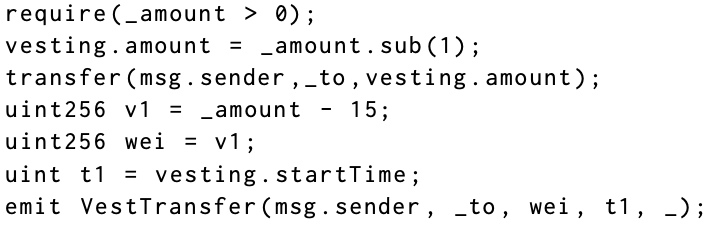
\includegraphics[scale=0.45]{stepOne}
    \caption{Method in Victim Program}
  \end{figure}
  \pause
  \begin{figure}
    \centering
  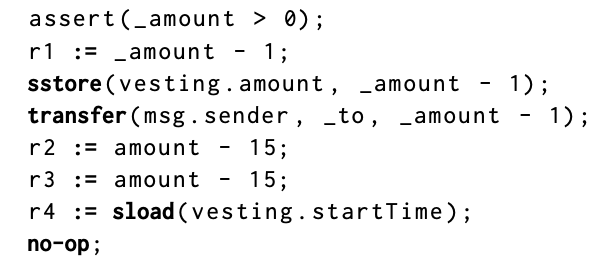
\includegraphics[scale=0.45]{stepTwo}
    \caption{Symbolic execution on $\Gamma_s$}
  \end{figure}
\end{frame}

\begin{frame}
  \frametitle{Summary Based Symbolic Execution}
  \framesubtitle{Example - \boldIt{Step 2}}
  \begin{figure}
    \centering
  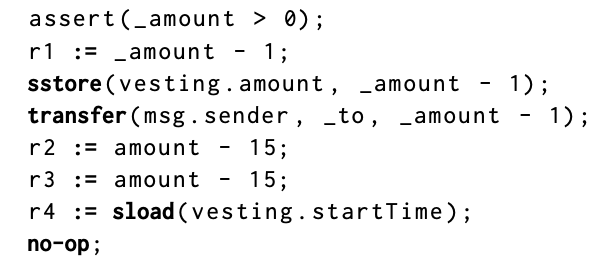
\includegraphics[scale=0.45]{stepTwo}
    \caption{Symbolic execution on $\Gamma_s$}
  \end{figure}
  \pause
  \begin{figure}
    \centering
  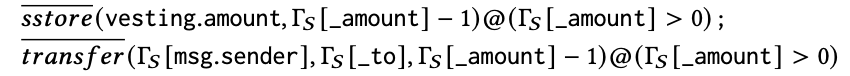
\includegraphics[scale=0.45]{stepThree}
    \caption{Summary Generation via \textit{get-summary}}
  \end{figure}
\end{frame}
\section{Summary Interpretation}
\begin{frame}
  \frametitle{Recap}
  \begin{itemize}
    \item Given \textit{Attack Program Synthesis} specification $(\Gamma_0, \mathcal{V}, \mathcal{S})$,
      Want to find a \textit{concrete program} $P$ such that:
      \begin{itemize}
        \item $\Gamma = \llbracket P \rrbracket_{\Gamma_0}$
        \item $\Gamma \vDash \mathcal{V}$.
      \end{itemize}
      \item Finding such a $P$ requires solving the SMT query $\exists \vect{v} .
        \mathcal{V}(\llbracket \mathcal{S} \rrbracket_{\Gamma_0})$
      \item $\mathcal{S}$ is a sequence of $k$-\textit{holes} of the form
        $\hole(f_1(v_{\tau_1}), f_2(v_{\tau_2}), \dots, f_n(v_{\tau_n}))$
    \item For each of the components $(f_i, \tau_i)$, SOLAR generated
      summary $(\overline{f_i}, \tau_i)$.
    \item Instead of symbolically executing $f_i(v_{\tau_i})$, use
      $\overline{f_i}(v_{\tau_i})$ via \textit{Summary Interpretation}.
  \end{itemize}
\end{frame}
\begin{frame}[fragile]
  \frametitle{Summary Interpretation}
    \begin{center}
      \begin{tabular}{c}
  \begin{lstlisting}[language=Racket,mathescape=true]
  (define (interpret-summary $s@\phi$ $\Gamma$)
    (define $s_{\Gamma}@\phi_{\Gamma}$ (substitute $s@\phi$ $\Gamma$))
    (match $s_{\Gamma}$
      [$\transfer(x_{\Gamma}, y_{\Gamma}, z_{\Gamma})$ (when $\phi_{\Gamma}$ $\textit{transfer}(x_{\Gamma}, y_{\Gamma}, z_{\Gamma})$) ]
      [$\sstore(x_, y_{\Gamma})$ (when $\phi_{\Gamma}$ $\textit{sstore}(x, y_{\Gamma})$) ]
      [_ noop]
    )
  )
  \end{lstlisting}
  \end{tabular}
    \end{center}

    \begin{itemize}
      \item Summary $s@\phi$ was generated over symbolic state $\Gamma_{s} = \{ x_1 \mapsto v_1, x_2
        \mapsto v_2, \dots, x_n \mapsto v_n \}$.
      \item Line 2 substitutes $v_i$ in $s@\phi$ with corresponding value
        $\Gamma[x_i]$ to give $s_{\Gamma}@\phi_{\Gamma}$ .
      \item On Lines 3-5, $s_\Gamma$ is \textit{interpreted} according to the standard
        semantics if $\phi_{\Gamma}$
      \item SOLAR only need to interpret state that change \textit{persistent state}.
    \end{itemize}
\end{frame}

\begin{frame}[fragile]
  \frametitle{SOLAR Algorithm}
    \begin{center}
      \begin{tabular}{c}
  \begin{lstlisting}[language=Racket,mathescape=true,basicstyle=\tiny]
  (define (solar $\mathcal{V}$ $\Upsilon$ $K$)
    (define $\mathcal{S}$ (for/list ([i $K$]) (apply choose* $\Upsilon$)))
    (define $\Gamma_0$ (get-initial-state $\Upsilon$))
    (define $\llbracket \mathcal{S} \rrbracket_{\Gamma_0}$ (interpret $\mathcal{S}$ $\Gamma_0$ ))
    (define binding (solve (assert ($\mathcal{V}$ $\llbracket \mathcal{S}
    \rrbracket_{\Gamma_0}$))))
    (evaluate program binding))
  \end{lstlisting}
  \end{tabular}
  \end{center}
  \begin{itemize}
    \item Line 2 constructs $\mathcal{S}$ as sequence of $K$ choose statements.
    \item Line 3 constructs $\Gamma_0$, the initial program state.
    \item Line 4 interprets $\mathcal{S}$ on $\Gamma_0$.
    \item Line 6 makes a call to the SMT solver to find $\Gamma$ that satisfies
      $\mathcal{V}$
  \end{itemize}
\end{frame}


\end{document}

